\part*{Lektion 9: SciPy und Matplotlib}
\section{SciPy}
\begin{itemize}
	\item Python-Bibliothek
	\item[\-] \texttt{from scipy import integrate}
	\item[\-] \texttt{from scipy import interpolate}
	\item[\-] \texttt{from scipy import optimize}
	\item[\-] \texttt{from scipy import signal}
	\item[\-] ...
	\item Basiert auf NumPy
	\item Enthält numerische Algorithmen und mathematische Werkzeuge\\
	\item \url{https://docs.scipy.org/doc/scipy/reference/}
\end{itemize}

\subsection{SciPy.Interpolate}
\begin{itemize}
	\item 1-dimensionale Interpolation
	\item Mehrdimensionale Interpolation
	\item Splines
	\item API-Referenz:
	\item[\-] \url{https://docs.scipy.org/doc/scipy/reference/interpolate.html}
\end{itemize}
\lstinputlisting{listings/v9_interpolate1.py}
Stützwerte für x und y:
\lstinputlisting{listings/v9_interpolate2.py}
Interpolationsfunktionen erstellen:
\lstinputlisting{listings/v9_interpolate3.py}
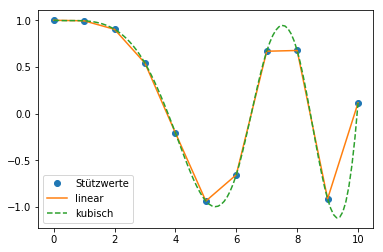
\includegraphics[width=0.4\linewidth]{images/v9_interpolate1}

\subsection{SciPy.Integrate}
\begin{itemize}
	\item Integration von gegebenen Funktionen
	\item Integration von diskreten Samples
	\item Numerische Integratoren für Differentialgleichungen (ODE)
	\item API-Referenz:
	\item[\-] \url{https://docs.scipy.org/doc/scipy/reference/integrate.html}
\end{itemize}
\lstinputlisting{listings/v9_integrate1.py}
Diskrete Samples:
\lstinputlisting{listings/v9_integrate2.py}
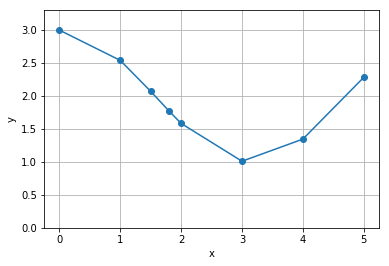
\includegraphics[width=0.4\linewidth]{images/v9_integrate1}
Integral (Fläche unter dem Graphen) berechnen:
\lstinputlisting{listings/v9_integrate3.py}
\textbf{Gegebene Funktion}
\lstinputlisting{listings/v9_integrate4.py}

\section{Matplotlib}
\begin{itemize}
	\item Tipps und Tricks in Jupyter
	\item Figure mit Subplots erstellen
	\item \texttt{plt.contour()} und \texttt{plt.contourf()}
	\item \texttt{plt.loglog()}
\end{itemize}

\subsection{Tipps für Jupyter-Notebook}
Folgende Zeile einfügen, damit man nicht immer \texttt{plt.show()} aufrufen muss
\lstinputlisting{listings/v9_matplotlib1.py}
Ein Semikolon am Zeilenende unterdrückt lästige Meldungen (\texttt{plt.plot(...);})

\subsection{Subplots}
Einzelne Subplots nacheinander erstellen:
\lstinputlisting{listings/v9_matplotlib2.py}
Alle Subplots von Anfang an erstellen:
\lstinputlisting{listings/v9_matplotlib3.py}

\subsection{Pyplot-Funktionen}
\subsubsection{Treppensignal}
\lstinputlisting{listings/v9_matplotlib4.py}
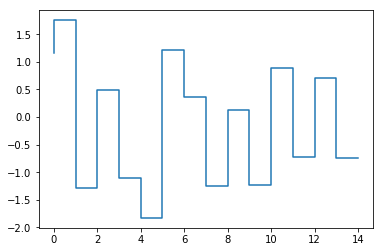
\includegraphics[width=0.4\linewidth]{images/v9_matplotlib1}

\subsubsection{\texttt{contourf()}}
\url{https://matplotlib.org/api/_as_gen/matplotlib.pyplot.contourf.html}\\
\url{https://matplotlib.org/tutorials/colors/colormaps.html}
\lstinputlisting{listings/v9_matplotlib5.py}
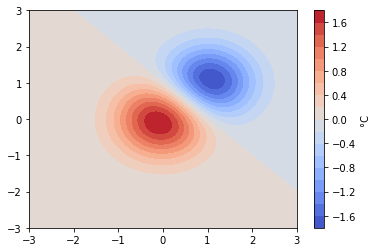
\includegraphics[width=0.4\linewidth]{images/v9_matplotlib2}

\subsubsection{\texttt{contour()}}
\url{https://matplotlib.org/api/_as_gen/matplotlib.pyplot.contour.html}
\lstinputlisting{listings/v9_matplotlib6.py}
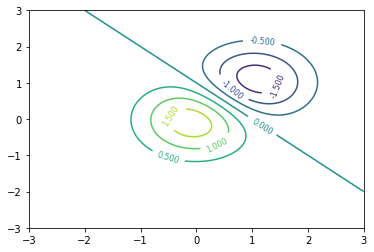
\includegraphics[width=0.4\linewidth]{images/v9_matplotlib3}

\subsubsection{\texttt{loglog()}}
\url{https://matplotlib.org/api/_as_gen/matplotlib.pyplot.loglog.html}
\lstinputlisting{listings/v9_matplotlib7.py}
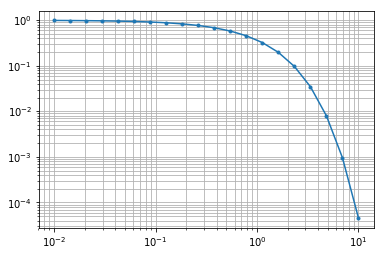
\includegraphics[width=0.4\linewidth]{images/v9_matplotlib4}

\subsubsection{XKCD}
\url{https://xkcd.com/}\\
\url{https://matplotlib.org/api/_as_gen/matplotlib.pyplot.xkcd.html}\\
\url{https://packages.debian.org/buster/fonts-humor-sans}\\
\url{https://github.com/shreyankg/xkcd-desktop/blob/master/Humor-Sans.ttf}
\lstinputlisting{listings/v9_matplotlib8.py}
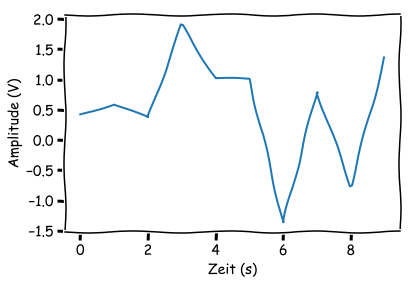
\includegraphics[width=0.4\linewidth]{images/v9_matplotlib5}